\subsection{整体 SOH 估计框架}

电池健康状态（state of health, SOH）是衡量电池退化程度的重要指标。尽管目前尚缺乏统一的 SOH 定义，但电池容量仍是最常用的表征方式之一\cite{ref13,ref14}。本文从容量衰减维度表征电池健康状态，并将当前可用容量与额定容量之比定义为 SOH：

\begin{equation}
\mathrm{SOH}=\frac{C_{\mathrm{current}}}{C_{\mathrm{rated}}}\times100\%,
\end{equation}

其中，$C_{\mathrm{current}}$ 和 $C_{\mathrm{rated}}$ 分别表示电池当前可用容量和额定容量。

本文所建立的 SOH 估计流程如\cref{fig:2-1}所示，具体步骤如下。

\begin{figure}[H]
\centering
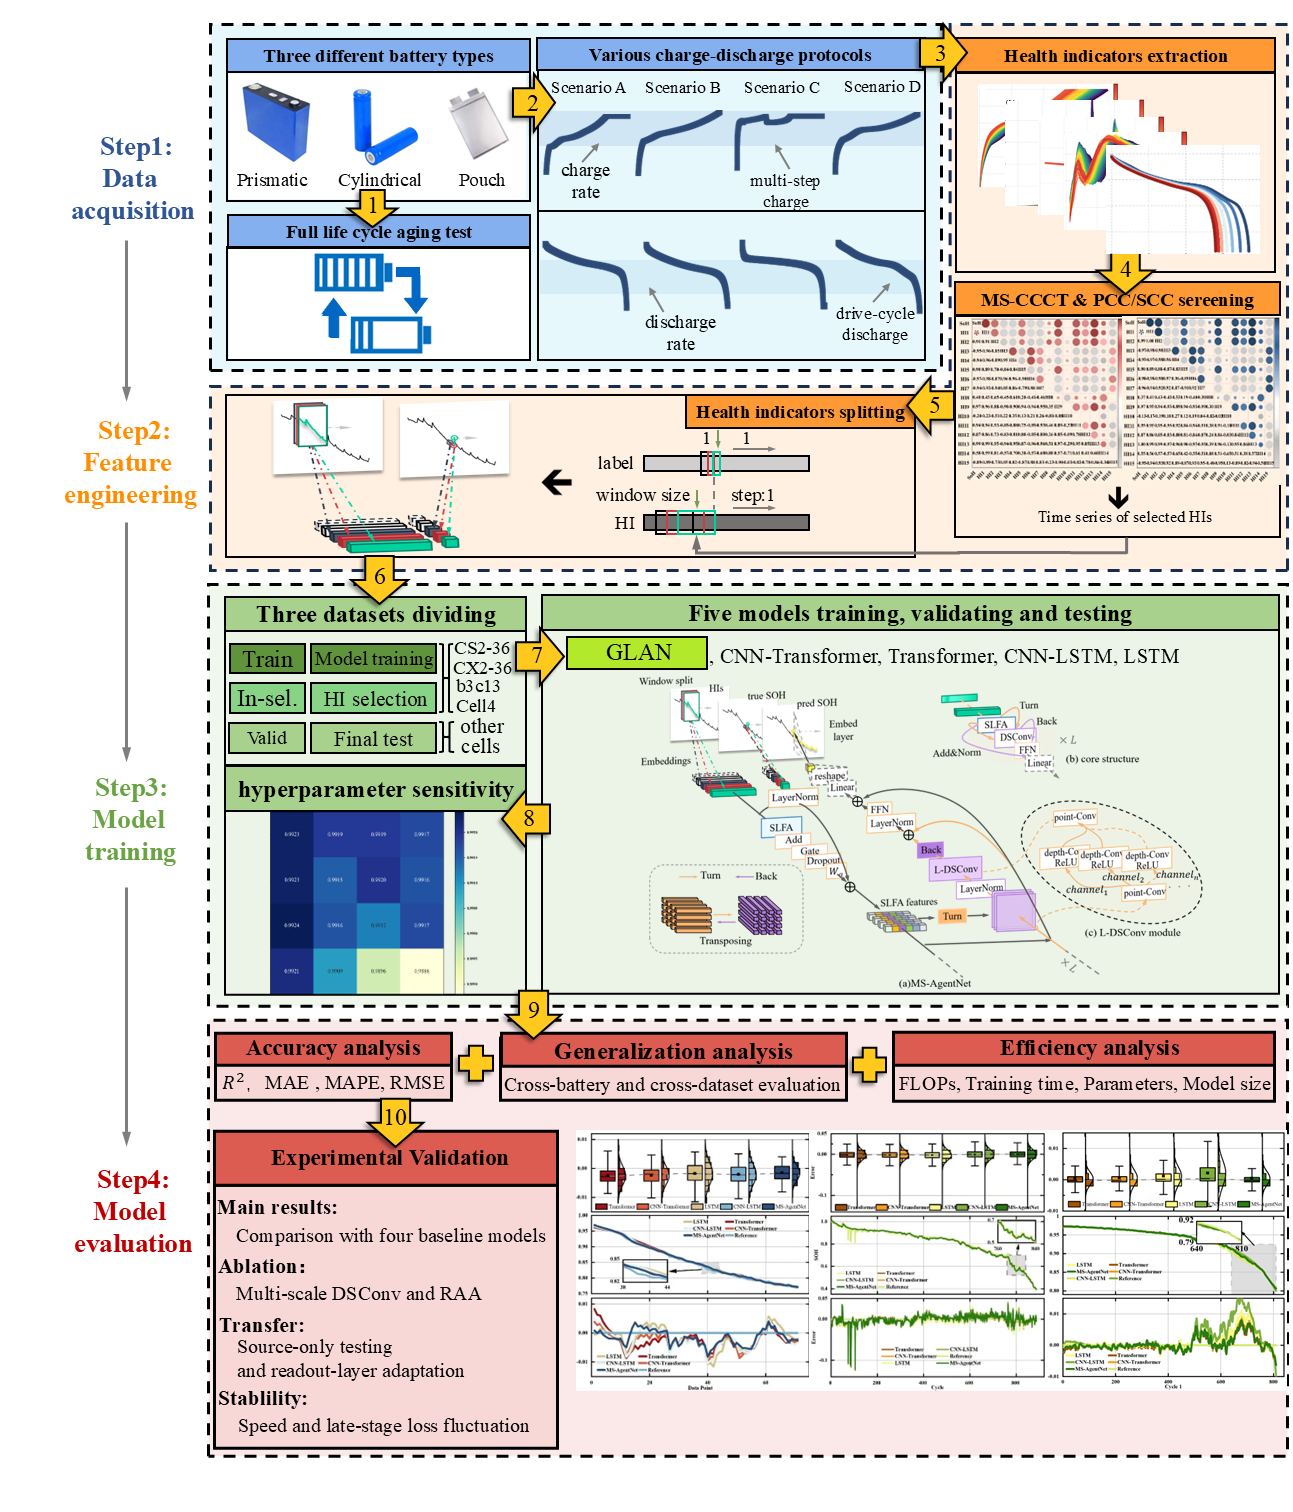
\includegraphics[width=0.70\textwidth]{figures/fig1.png}
\caption{Flowchart of the developed SOH estimation approach.}
\label{fig:2-1}
\end{figure}


（1）\textbf{数据获取。} 选取不同材料体系和运行工况下的公开电池老化数据，获取循环过程中的电压、电流、时间和容量等信息，并提取相应充放电过程数据，为健康指标构建和 SOH 估计提供数据基础。

（2）\textbf{健康指标构建。} 从电池充放电过程中提取候选健康指标，利用 MS-CCCT 标定 CCCT 电压窗口，并结合 PCC/SCC 双阈值与冗余约束筛选模型输入。随后，采用滑动窗口将健康指标时间序列划分为输入样本，窗口每次向前移动一个循环，并将窗口后紧邻循环的真实 SOH 作为对应标签。

（3）\textbf{模型训练。} 将构建的健康指标序列输入所提出的 MS-AgentNet，利用训练电池进行模型参数学习，并根据预先指定的配置选择电池确定模型配置。配置确定后保持冻结，并直接在独立评价电池上进行测试，以考察模型的跨电池估计性能。

（4）\textbf{性能评价。} 从估计精度、计算效率和模型稳定性等方面评价所提方法，并与多种 SOH 估计模型进行比较。

\subsection{典型电池数据集}

公开电池老化数据为 SOH 估计方法的复现与横向比较提供了重要基础。为评估所提方法在不同电池体系和运行条件下的估计性能，选取 Oxford、CALCE CS2、CALCE CX2 和 MIT/Severson 四组公开电池老化数据进行实验。这些数据由牛津大学电池智能实验室、马里兰大学先进生命周期工程中心以及 MIT、Stanford University 和 Toyota Research Institute 等研究机构发布，具有规范的实验协议和较为完整的数据记录。四组数据在电芯类型、材料体系、容量规格、测试温度和充放电协议等方面存在差异，可用于考察所提方法在不同退化条件下的适用性与估计性能。各数据集的主要实验信息汇总于\cref{tab:2-1}；\cref{fig:2-2}(a)--(d)展示了四组数据中所选电池的容量衰减曲线，\cref{fig:2-2}(e)--(h)展示了各数据集中代表性电池在不同 SOH 水平下的充电电压曲线。

\begin{table}[!htbp]
\caption{Description of the four battery datasets.}
\label{tab:2-1}
\centering
\fontsize{9.5pt}{12pt}\selectfont
\setlength{\tabcolsep}{4pt}
\renewcommand{\arraystretch}{1.12}
\begin{tabularx}{\linewidth}{@{}
>{\raggedright\arraybackslash}p{0.205\linewidth}
>{\hsize=0.86\hsize\linewidth=\hsize\raggedright\arraybackslash}X
>{\hsize=0.97\hsize\linewidth=\hsize\raggedright\arraybackslash}X
>{\hsize=0.97\hsize\linewidth=\hsize\raggedright\arraybackslash}X
>{\hsize=1.20\hsize\linewidth=\hsize\raggedright\arraybackslash}X@{}}
\toprule
Data Sources & Oxford \cite{ref60} & CALCE CS2 \cite{ref18,ref61} & CALCE CX2 \cite{ref18,ref61} & MIT/Severson \cite{ref62} \\
\midrule
Manufacturer & Kokam & LG Chem & LG Chem & A123 Systems \\
\addlinespace[2pt]
Cell types & Pouch & Prismatic & Prismatic & 18650 cylindrical \\
\addlinespace[2pt]
Cathode material & NCO-LCO & LCO & LCO & LFP \\
\addlinespace[2pt]
Rated capacity (Ah) & 0.74 & 1.10 & 1.35 & 1.10 \\
\addlinespace[2pt]
Capacity failure\newline threshold & 70\% & 0.84 Ah (76.4\%) & 1.08 Ah (80\%) & 80\% \\
\addlinespace[4pt]
Charge protocol\newline (rate) & CC (2C) & CC-CV\newline (0.5C, 4.2 V) & CC-CV\newline (0.5C, 4.2 V) & Two-step fast charge\newline + CC-CV (1C, 3.6 V) \\
\addlinespace[3pt]
Discharge protocol\newline (rate) & variance & CC (1C) & CC (1C) & CC (4C) \\
\addlinespace[3pt]
Cut-off voltage (V) & charge to 4.2\newline discharge to 2.7 & charge to 4.2\newline discharge to 2.7 & charge to 4.2\newline discharge to 2.7 & charge to 3.6\newline discharge to 2.0 \\
\addlinespace[3pt]
Cut-off current (A) & --- & charge to 0.05 & charge to 0.05 & charge to 0.022\newline (C/50) \\
\addlinespace[3pt]
Experiment\newline temperature ($^\circ$C) & 40 & 24 & 24 & 30 \\
\bottomrule
\end{tabularx}
\end{table}


\begin{figure}[!htb]
\centering
\noindent\makebox[\linewidth][c]{%
  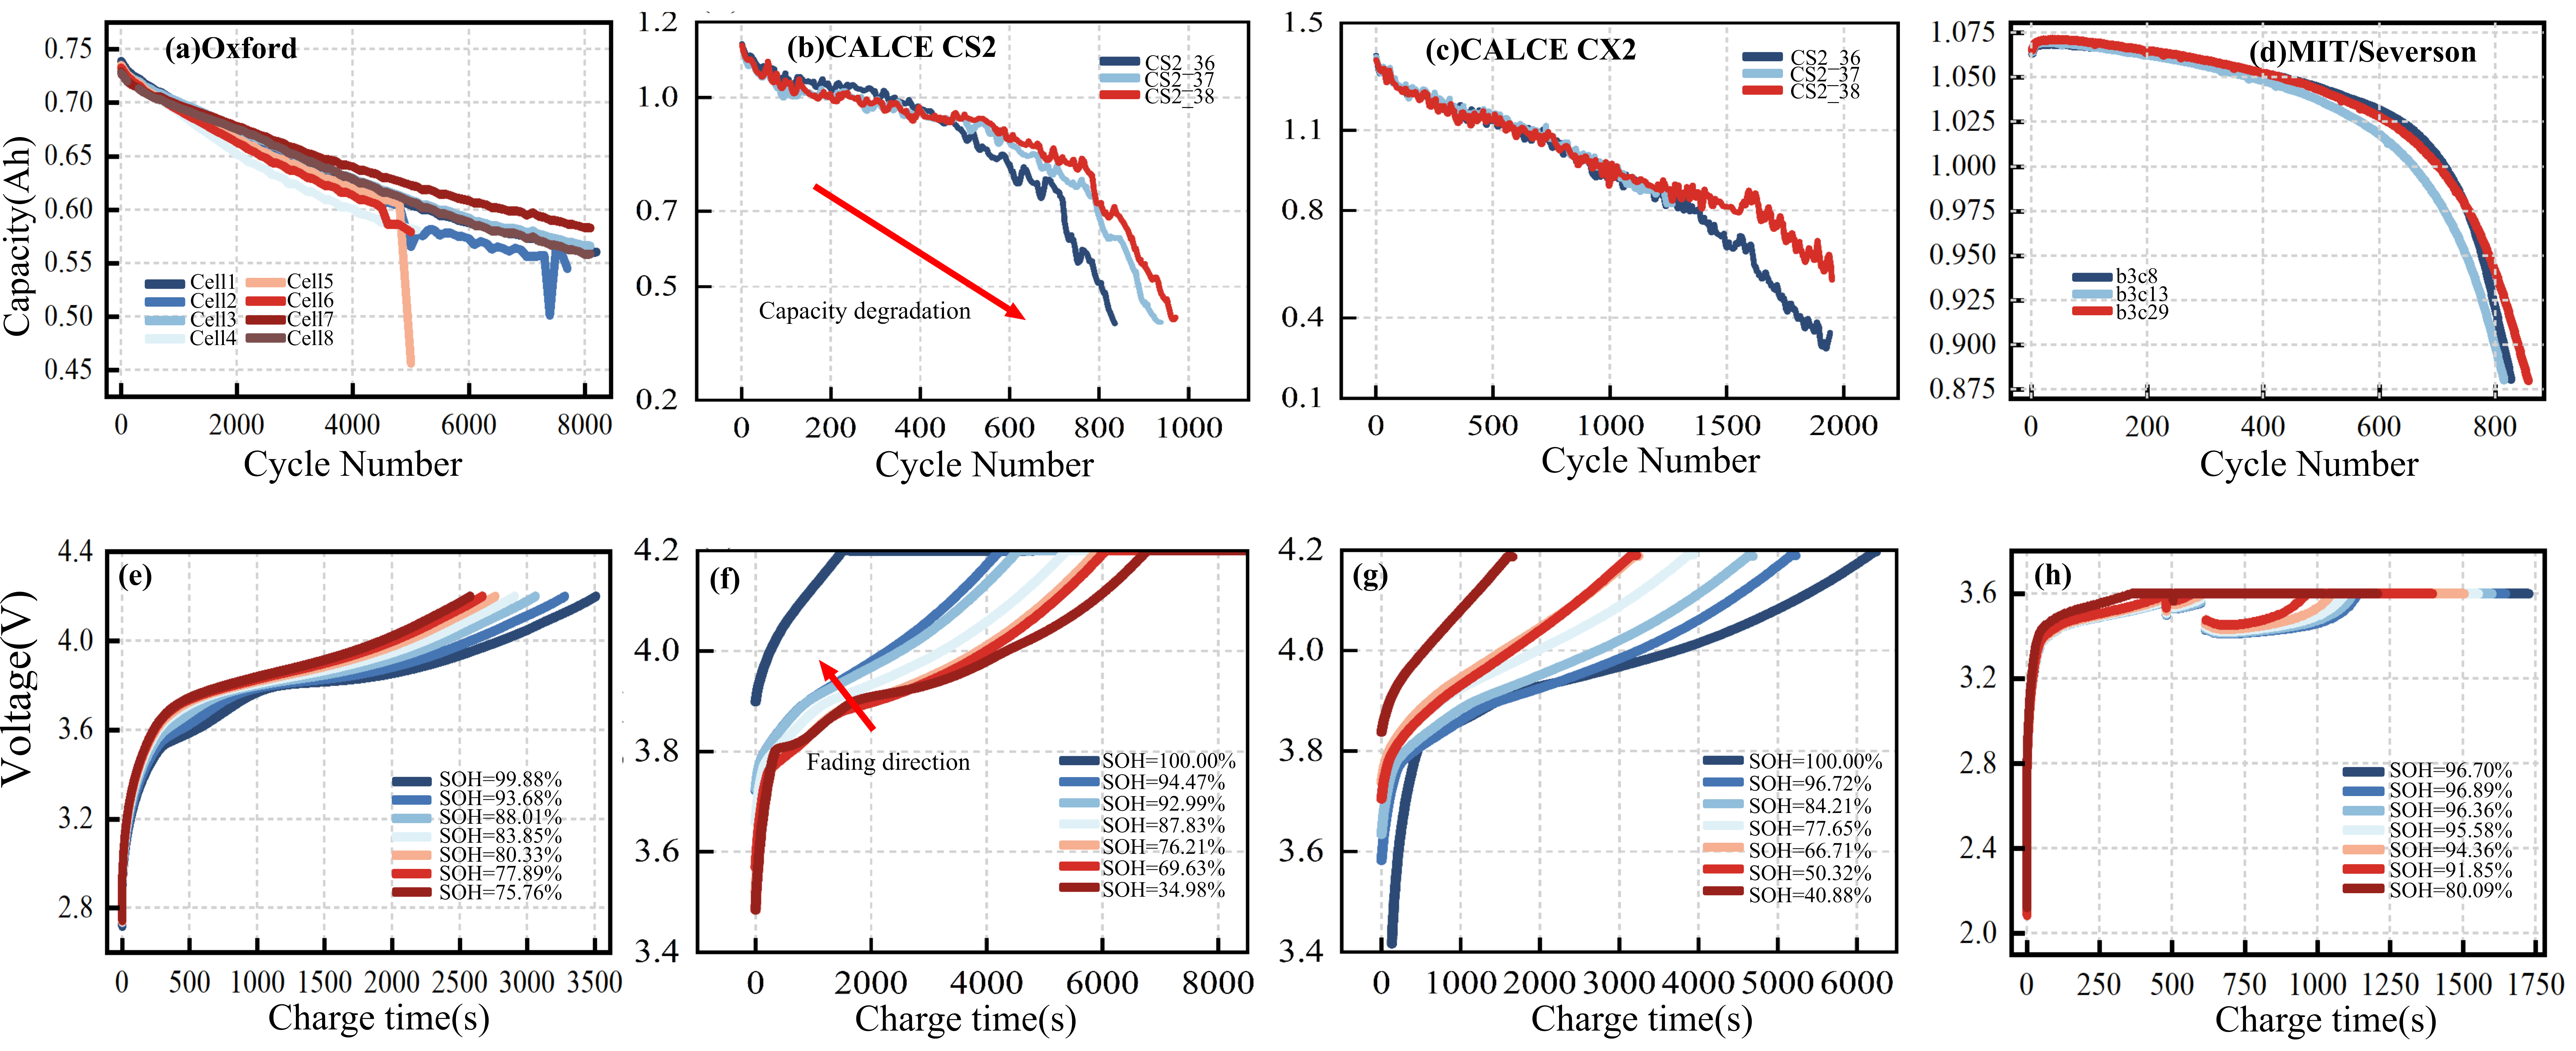
\includegraphics[width=175mm,trim=0 10 10 10,clip]{figures/fig2.png}%
}
\caption{Four battery datasets: (a)--(d) capacity degradation curves of Oxford, CALCE CS2, CALCE CX2, and MIT/Severson cells, respectively; (e)--(h) charging voltage curves of the four datasets in the same order.}
\label{fig:2-2}
\end{figure}


\subsubsection{Oxford 锂离子电池数据集}

Oxford 数据集由牛津大学电池智能实验室提供，包含 8 节 Kokam SLPB533459H4 锂离子软包电池\cite{ref28}。电池负极采用石墨材料，正极为 NCO-LCO 混合体系\cite{ref60}，标称容量为 0.74 Ah，老化实验在 40 ℃ 条件下进行。充电过程采用 CC-CV 协议充至 4.2 V，随后按照源自城市 ARTEMIS 工况的动态电流曲线放电至 2.7 V\cite{ref28,ref61}。选取 Cell1–Cell8 的循环老化数据进行实验。

\subsubsection{CALCE 锂离子电池数据集}

CALCE CS2 与 CX2 数据集均来源于马里兰大学先进生命周期工程中心（CALCE）\cite{ref18,ref61}。两组电池均为采用 LCO 正极材料的方形锂离子电池，标称容量分别约为 1.1 Ah 和 1.35 Ah，老化实验在约 24 ℃ 条件下开展。依据下载的 CALCE 原始数据记录，两组电池均采用 CC-CV 充电协议，以 0.5C 恒流充电至 4.2 V，随后保持恒压直至充电电流降至 0.05 A；选用的 CS2\_36–CS2\_38 和 CX2\_36–CX2\_38 均以 1C 恒流方式放电至 2.7 V。

\subsubsection{MIT/Severson 锂离子电池数据集}

MIT/Severson 数据集由 MIT、Stanford University 和 Toyota Research Institute 联合发布\cite{ref62}，包含 A123 APR18650M1A 型 18650 圆柱锂离子电池。该系列采用 LFP/石墨体系，标称容量约为 1.1 Ah，老化实验在 30 ℃ 条件下进行。充电采用一步或两步快速充电策略，其中两步策略按照 $C_1(Q_1)-C_2$ 方式以不同恒流倍率充至 80\% SOC，随后以 1C CC-CV 方式完成充电；放电过程采用 4C 恒流方式，截止电压为 2.0 V。选取 b3c8、b3c13 和 b3c29 三节电池，其中 b3c8 采用 5.3C(54\%)–4C 充电策略，b3c13 和 b3c29 采用 5.6C(36\%)–4.3C 充电策略。

\subsection{特征工程}

本节从充放电数据中构建多源候选健康指标，其中 CCCT 的电压窗口由 MS-CCCT 依据多节特征开发电池的相关性评价结果进行标定。窗口确定后，结合候选指标与 SOH 的关联程度及指标间的冗余关系，确定各数据集的模型输入。

\subsubsection{健康指标提取}

本文从充电时间、增量容量、温度微分及局部充放电区间等特征类型\cite{ref52,ref63,ref64,ref65}出发，由充放电数据构建包含 15 项健康指标的候选池。充电侧候选健康指标包括由充电电压–时间（CVT）、增量容量（IC）、微分温度–电压（DTV）和微分温度–容量（DTC）曲线提取的时长、幅值、特征位置和分布宽度，放电侧候选健康指标包括窗口放电容量和能量效率，各指标的分类与定义见\cref{tab:2-2}。

充电电压–时间曲线记录恒流充电阶段端电压随时间的变化，可由电压与时间采样直接获得。随着循环推进，CVT 曲线在时间轴上的位置逐渐变化（\cref{fig:2-3}(b)），说明同一电压区间内的充电时长包含与容量衰减相关的信息，因此可从中提取恒流充电时间作为候选健康指标\cite{ref63,ref64}。据此定义 CCCT：

\begin{equation}
CCCT(V_l,V_h)=t(V_h)-t(V_l),
\end{equation}

其中，$t(V_l)$、$t(V_h)$ 分别表示充电电压达到窗口上下边界的时刻。CCCT 的电压窗口由 MS-CCCT 进行标定，标定后得到的窗口充电时间记为 HI1。

除充电时序特征外，容量随电压的变化同样蕴含退化信息。增量容量（IC）曲线是解析电池电化学退化的经典分析手段。该方法对容量关于电压求导，将平缓的充电电压平台转化为辨识度更高的特征峰，其位置与形状随老化发生变化\cite{ref50,ref64}。IC、DTV 和 DTC 均通过采样序列的差分近似计算，微分运算容易放大采样噪声\cite{ref28,ref50}。因此，在差分计算前对相应序列进行滑动平均处理，滤波窗口设为 200 个采样点。IC 的具体表达式为：

\begin{equation}
IC=\frac{dQ}{dV}\approx\frac{Q_{k+N}-Q_k}{V_{k+N}-V_k},
\end{equation}

其中，$V_k$、$Q_k$ 为第 $k$ 个采样点的端电压和充电容量，$N$ 为两个采样点之间的间隔。不同循环下 IC 曲线的峰值、特征位置和分布宽度随老化发生变化（\cref{fig:2-3}(a)），本文分别提取峰值、峰值对应电压和半峰宽，并将其定义为 HI2、HI3 和 HI4。

温度是反映电池内部状态的另一重要维度。恒流充电过程中，电池表面温度变化通常较为缓慢，老化带来的微小热响应差异难以通过原始温度曲线直接识别。微分温度–电压（DTV）曲线由 Wu 等人\cite{ref65}提出，通过计算充电过程中电池表面温度相对电压的变化率，将热响应映射至电压域，并形成随老化变化的峰谷特征曲线\cite{ref64,ref65}。其定义如下：

\begin{equation}
DTV=\frac{dT}{dV}\approx\frac{T_{k+N}-T_k}{V_{k+N}-V_k},
\end{equation}

其中，$V_k$、$T_k$ 为第 $k$ 个采样点的端电压和电池表面温度，$N$ 为两个采样点之间的间隔。

不同循环下 DTV 曲线的峰谷幅值与特征位置呈现相应变化（\cref{fig:2-3}(c)）。本文从中提取峰值（HI5）、峰值对应电压（HI6）、谷值（HI7）、谷值对应电压（HI8）和峰谷差（HI9），分别描述热响应的幅值、特征位置及波动范围\cite{ref64}。

与 DTV 在电压域刻画热响应不同，DTC 在充电容量域刻画热响应。DTC 以充电容量为自变量，描述温度变化率随容量的演化，其定义如下\cite{ref64}：

\begin{equation}
DTC=\frac{dT}{dQ}\approx\frac{T_{k+N}-T_k}{Q_{k+N}-Q_k},
\end{equation}

其中，$T_k$、$Q_k$ 为第 $k$ 个采样点的电池表面温度和充电容量，$N$ 为两个采样点之间的间隔。\cref{fig:2-3}(d)所示 DTC 曲线同样表现出随循环变化的峰值、特征位置和分布宽度，本文据此提取峰值、峰值对应容量和半峰宽，并将其定义为 HI10、HI11 和 HI12。

放电侧从容量保持与能量转换两个角度补充退化信息。放电容量指端电压由上限 $V_h$ 降至下限 $V_l$ 时释放的电荷量。该电荷量可由放电电流对时间的积分获得：

\begin{equation}
Q_{\mathrm{dch}}(V_h,V_l)=\frac{1}{3600}\int_{\tau(V_h)}^{\tau(V_l)}\left|I_{\mathrm{dch}}(t)\right|\,dt,
\end{equation}

其中，$\tau(V_h)$ 与 $\tau(V_l)$ 分别表示放电过程中端电压达到上下限的时刻，$|I_{\mathrm{dch}}(t)|$ 为放电电流幅值，时间 $t$ 以 s 为单位，$Q_{\mathrm{dch}}$ 的单位为 Ah。若放电过程中端电压多次穿越同一电压边界，则对该电压区间内的电流进行累计积分。本文进一步构造两个窗口放电容量候选指标，分别计算端电压由 3.80 V 降至 3.40 V 以及由 3.20 V 降至 3.00 V 过程中释放的电荷量，并记为 HI13 和 HI14\cite{ref31,ref52}。

能量效率反映电池在充放电过程中的能量转换特性，定义为单次循环放电能量与充电能量之比\cite{ref66}：

\begin{equation}
\eta=\frac{E_{\mathrm{dch}}}{E_{\mathrm{ch}}}=\frac{\int_0^{t_{\mathrm{dch}}}V_{\mathrm{dch}}(t)\left|I_{\mathrm{dch}}(t)\right|\,dt}{\int_0^{t_{\mathrm{ch}}}V_{\mathrm{ch}}(t)\left|I_{\mathrm{ch}}(t)\right|\,dt},
\end{equation}

其中，$V_{\mathrm{ch}}(t)$、$|I_{\mathrm{ch}}(t)|$、$t_{\mathrm{ch}}$ 与 $V_{\mathrm{dch}}(t)$、$|I_{\mathrm{dch}}(t)|$、$t_{\mathrm{dch}}$ 分别表示充电与放电阶段的端电压、电流幅值和持续时间，充电与放电均取完整循环过程。该能量效率记为 HI15（$\eta$）。

\subsubsection{组级双相关 MS-CCCT}

已有研究常从预设充电电压区间提取 CCCT 或局部充电特征\cite{ref28,ref63}，也有研究通过电压区间优化或逐级细化窗口提高特征相关性\cite{ref31,ref51}。然而，不同电池体系的退化敏感电压区间存在差异，固定窗口可能遗漏与 SOH 密切相关的局部退化信息，从而影响健康指标的跨电池稳定性。对于每个数据集，将训练电池和配置选择电池共同组成特征开发电池集合 $\mathcal{B}$，用于 CCCT 电压窗口标定和健康指标筛选；独立评价电池不属于该集合。本文在覆盖相应充电电压范围的搜索区间内构建多尺度扫描窗口，并利用集合内各电池的 PCC 和 SCC 自适应标定最优 CCCT 区间。

为比较不同候选窗口的有效性，需要量化窗口特征与 SOH 之间的相关性。本文同时采用皮尔逊相关系数（PCC）和斯皮尔曼相关系数（SCC）作为评价依据：PCC 衡量线性相关强度，SCC 衡量单调相关强度，二者可分别反映线性退化趋势和单调非线性退化特征\cite{ref25,ref53,ref55}。第 $i$ 个候选窗口在第 $j$ 个特征开发电池上的 PCC $\gamma_{i,j}$ 和 SCC $\rho_{i,j}$ 定义为

\begin{equation}
\gamma_{i,j}=
\frac{\displaystyle\sum_{k=1}^{n_j}(f_{i,j,k}-\bar{f}_{i,j})(y_{j,k}-\bar{y}_j)}
     {\displaystyle\sqrt{\sum_{k=1}^{n_j}(f_{i,j,k}-\bar{f}_{i,j})^2\sum_{k=1}^{n_j}(y_{j,k}-\bar{y}_j)^2}},
\end{equation}

\begin{equation}
\rho_{i,j}=
\frac{\displaystyle\sum_{k=1}^{n_j}\bigl(R(f_{i,j,k})-\bar{R}(f_{i,j})\bigr)\bigl(R(y_{j,k})-\bar{R}(y_j)\bigr)}
{\displaystyle\sqrt{\sum_{k=1}^{n_j}\bigl(R(f_{i,j,k})-\bar{R}(f_{i,j})\bigr)^2\sum_{k=1}^{n_j}\bigl(R(y_{j,k})-\bar{R}(y_j)\bigr)^2}},
\end{equation}

式中，$f_{i,j,k}$ 表示第 $j$ 个特征开发电池上第 $i$ 个候选窗口在第 $k$ 个循环的特征值，$y_{j,k}$ 为对应循环的 SOH，$n_j$ 为第 $j$ 个特征开发电池的有效循环数。$\bar{f}_{i,j}$ 与 $\bar{y}_j$ 分别表示该电池上特征值与 SOH 的均值。$R(\cdot)$ 表示取秩操作，$\bar{R}(\cdot)$ 为对应秩序列的均值。$|\gamma_{i,j}|$ 越接近 1，说明线性关联越强；$|\rho_{i,j}|$ 越接近 1，说明单调关联越强。

为评价候选窗口在特征开发电池集合中的共同适用性，将第 $i$ 个候选窗口的最小绝对 PCC 和最小绝对 SCC 分别记为 $mPCC_i=\min_{j\in\mathcal{B}}|\gamma_{i,j}|$ 和 $mSCC_i=\min_{j\in\mathcal{B}}|\rho_{i,j}|$，并以二者中的较小值定义组级稳健得分：

\begin{equation}
S_i=\min_{j\in\mathcal{B}}\left\{\min\left(|\gamma_{i,j}|,\;|\rho_{i,j}|\right)\right\}.
\end{equation}

该得分由候选窗口在全部特征开发电池上的最低相关性决定。只有当窗口特征在各特征开发电池上均与 SOH 保持较强的线性和单调关联时，才能获得较高的 $S_i$。

MS-CCCT 采用由粗到细的多尺度搜索方式确定 CCCT 窗口\cite{ref31}。各阶段均以 $S_i$ 作为窗口比较依据，并将当前阶段得分最高的窗口作为下一阶段的搜索区域。

搜索过程分为三个阶段。R1 阶段以 0.40 V 窗宽和 0.20 V 步长进行粗粒度扫描，将 $S_i$ 最高的窗口作为父区域。R2 阶段在父区域内以 0.20 V 窗宽和 0.05 V 步长细化窗口。R3 阶段进一步以 0.10 V 窗宽和 0.05 V 步长考察更窄窗口能否提升相关性。若细化窗口的最高 $S_i$ 未超过父窗口，则停止细化并保留父窗口。按照这一搜索过程，四个数据集分别获得不同的 CCCT 窗口（\cref{tab:2-3}），说明退化敏感区间随数据集而变化，需要根据特征开发电池进行标定；各窗口的组级稳健得分均超过 0.98，表明相应 CCCT 在全部特征开发电池上均与 SOH 保持较强的线性和单调关联。

\subsubsection{健康指标筛选}

在 MS-CCCT 确定 HI1 的 CCCT 电压窗口后，进一步对 15 项候选健康指标执行统一的准入与冗余剔除。本文继续采用前述 PCC 和 SCC，分别评价候选健康指标与 SOH 之间的线性和单调关联，并考察候选指标之间的相关关系。上述相关系数均在每节特征开发电池上分别计算。

以 Oxford 数据集为例，\cref{fig:2-4}给出了 Cell1 和 Cell2 上 SOH 与 15 项候选健康指标以及候选指标之间的 PCC 和 SCC，其中矩阵下三角列出带符号的相关系数，上三角以圆圈大小和颜色深浅表示相关系数的绝对值。同一候选指标在两节电池上的相关强度并不完全一致：HI5（DTV 峰值）在 Cell1 上的 $|PCC|$ 和 $|SCC|$ 分别为 0.949 和 0.966，在 Cell2 上则降至 0.898 和 0.902，而 HI1 在两节电池上均保持较高相关性；同时，部分候选指标之间也具有较强的 PCC 和 SCC。前一现象说明单节电池上的高相关性未必能够延续至同组其他电池，后一现象则表明候选池中存在高度相关的信息，因而健康指标筛选需要同时考察跨电池相关性与指标间冗余。

针对上述两类情况，本文构建 PCC/SCC 双阈值—冗余约束健康指标筛选算法。该算法包括候选准入和冗余剔除两个阶段：在候选准入阶段，分别以 $\theta_{\mathrm{mono}}$ 和 $\theta_{\mathrm{lin}}$ 约束候选指标在全部特征开发电池上的最小 SCC 和最小 PCC，只有同时满足两项条件的指标才能进入候选集合，并按照 $R_i=\max(mPCC_i,mSCC_i)$ 确定考察顺序；在冗余剔除阶段，依次计算候选指标与已入选指标之间的组平均绝对 PCC 和 SCC，当两项相关系数均达到 $\theta_{\mathrm{co}}$ 时，将该候选指标判定为冗余。三个阈值在模型开发阶段预先设定，并在四个数据集的筛选过程中保持不变，完整流程见\cref{alg:2-1}。

按照\cref{alg:2-1}，Oxford 和 CS2 最终保留充电侧候选指标，其中二者均入选 HI1，CS2 进一步入选 HI2；CX2 入选窗口放电容量 HI13，MIT/Severson 入选窗口放电容量 HI14 和能量效率 HI15（\cref{tab:2-4}）。相同筛选规则在四个数据集上形成不同的健康指标组合，说明候选指标的有效性与具体电池数据有关。为考察这些指标在特征开发电池之外的稳定性，在保持其定义和参数不变的条件下，进一步计算各指标在独立评价电池上的 PCC 和 SCC（\cref{tab:2-5}）。Oxford Cell3–Cell8 上 HI1 的 $|\gamma|$ 和 $|\rho|$ 均高于 0.997，其余三个数据集独立评价电池上的最低 $|\gamma|$ 和 $|\rho|$ 分别为 0.932937 和 0.974359，表明最终入选指标在各自数据集的未见电池上仍保持较强的线性和单调关联。

除跨电池稳定性外，所选指标相对于已有健康指标的相关水平也是评价其有效性的依据。以能够获得逐电池文献结果的 Oxford 数据集为例，将本文 HI1 与样本熵、DTV/IC 特征及充电电压曲线斜率进行比较（\cref{tab:2-6}）。HI1 在 Cell3–Cell8 上的 $|\mathrm{PCC}|$ 为 0.997874–0.999337，且均高于所列文献在相应电池上的已报道值，表明 MS-CCCT 所确定的充电时间指标在 Oxford 独立评价电池上具有较强且稳定的 SOH 线性关联。

\begin{table}[!htbp]
\caption{Definitions of the candidate HIs.}
\label{tab:2-2}
\centering
\zihao{6}
\setlength{\tabcolsep}{2.0pt}
\renewcommand{\arraystretch}{1.12}
\begin{ThreePartTable}
\begin{tabularx}{0.98\linewidth}{
>{\centering\arraybackslash}p{0.045\linewidth}
>{\centering\arraybackslash}p{0.105\linewidth}
>{\raggedright\arraybackslash}X
>{\centering\arraybackslash}p{0.045\linewidth}
>{\centering\arraybackslash}p{0.105\linewidth}
>{\raggedright\arraybackslash}X}
\toprule
No. & Category & Health indicator & No. & Category & Health indicator \\
\midrule
HI1 & CVT & MS-CCCT 标定电压区间内的恒流充电时间
& HI9 & DTV & 微分温度--电压曲线的峰谷差 \\
HI2 & IC & 增量容量曲线的峰值
& HI10 & DTC & 微分温度--容量曲线的峰值 \\
HI3 & IC & 增量容量峰值对应的电压
& HI11 & DTC & 微分温度--容量曲线峰值对应的容量 \\
HI4 & IC & 增量容量特征峰的半峰宽
& HI12 & DTC & 微分温度--容量特征峰的半峰宽 \\
HI5 & DTV & 微分温度--电压曲线的峰值
& HI13 & 窗口放电容量 & 电压范围 3.80--3.40 V 内的放电容量 \\
HI6 & DTV & 微分温度--电压曲线峰值对应的电压
& HI14 & 窗口放电容量 & 电压范围 3.20--3.00 V 内的放电容量 \\
HI7 & DTV & 微分温度--电压曲线的谷值
& HI15 & 能量效率 & 单次循环放电能量与充电能量之比 \\
HI8 & DTV & 微分温度--电压曲线谷值对应的电压
& & & \\
\bottomrule
\end{tabularx}
\end{ThreePartTable}
\end{table}


\begin{figure}[htbp]
\centering
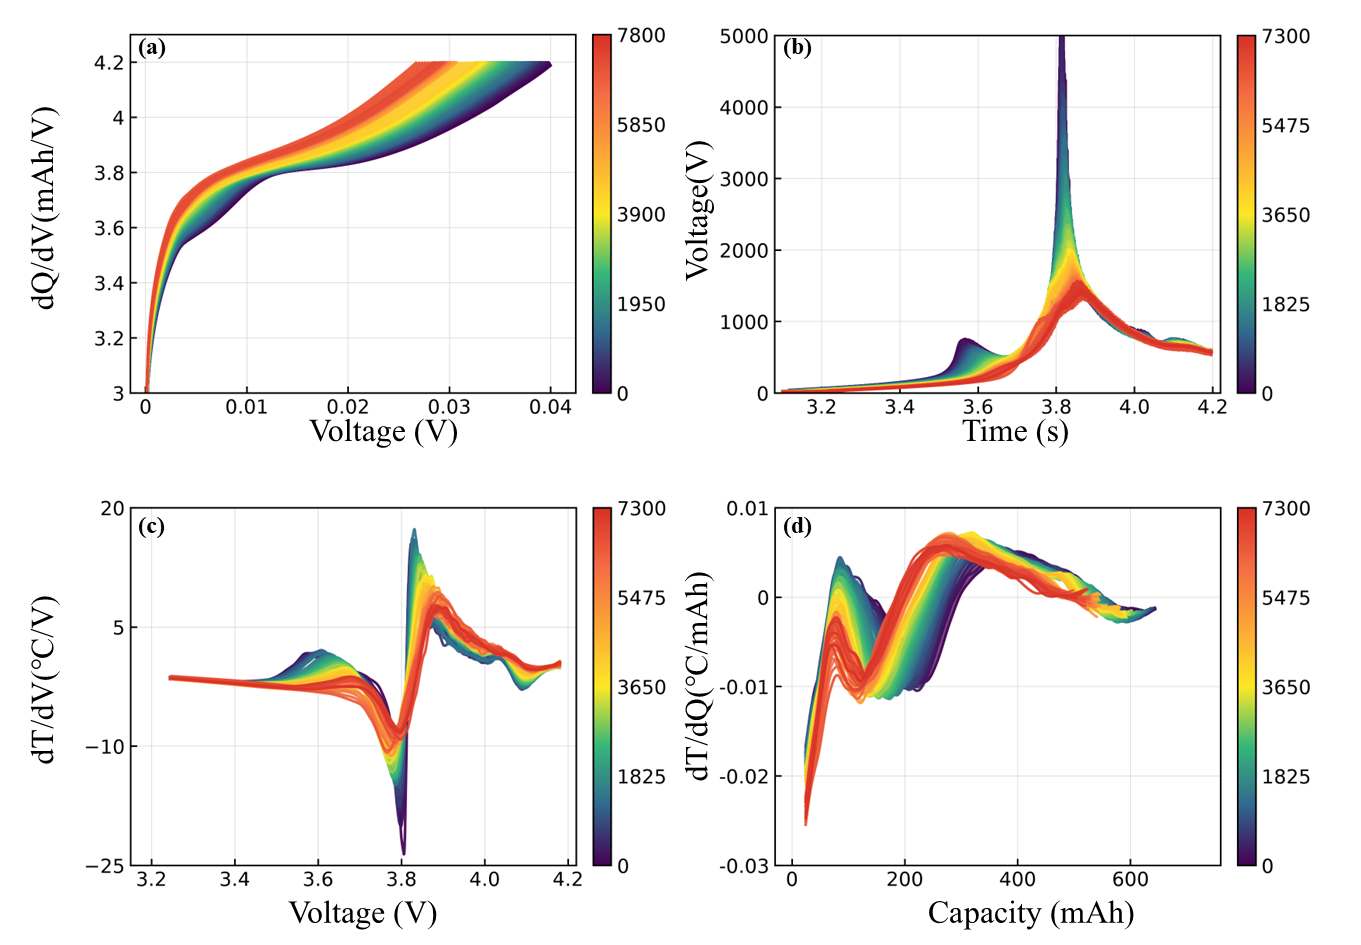
\includegraphics[width=0.92\textwidth]{figures/fig3.png}
\caption{Charge-side characteristic curves used for HI construction.}
\label{fig:2-3}
\end{figure}


\begin{table}
\TableStyle
\caption{Calibration results of the MS-CCCT window.}
\label{tab:2-3}
\begin{tabularx}{\linewidth}{@{\extracolsep{\fill}}L{1.10}C{1.50}C{0.80}C{0.80}C{0.80}@{}}
\toprule
Dataset & MS-CCCT window (V) & $mPCC$ & $mSCC$ & $S_i$ \\
\midrule
Oxford & 3.55–3.75 & 0.997322 & 0.994447 & 0.994447 \\
CS2 & 3.80–4.00 & 0.990286 & 0.980124 & 0.980124 \\
CX2 & 3.85–4.05 & 0.985921 & 0.990832 & 0.985921 \\
MIT/Severson & 2.970–3.170 & 0.995272 & 0.994419 & 0.994419 \\
\bottomrule
\end{tabularx}
\end{table}


\begin{figure}[!htb]
\centering
\noindent\makebox[\linewidth][c]{%
  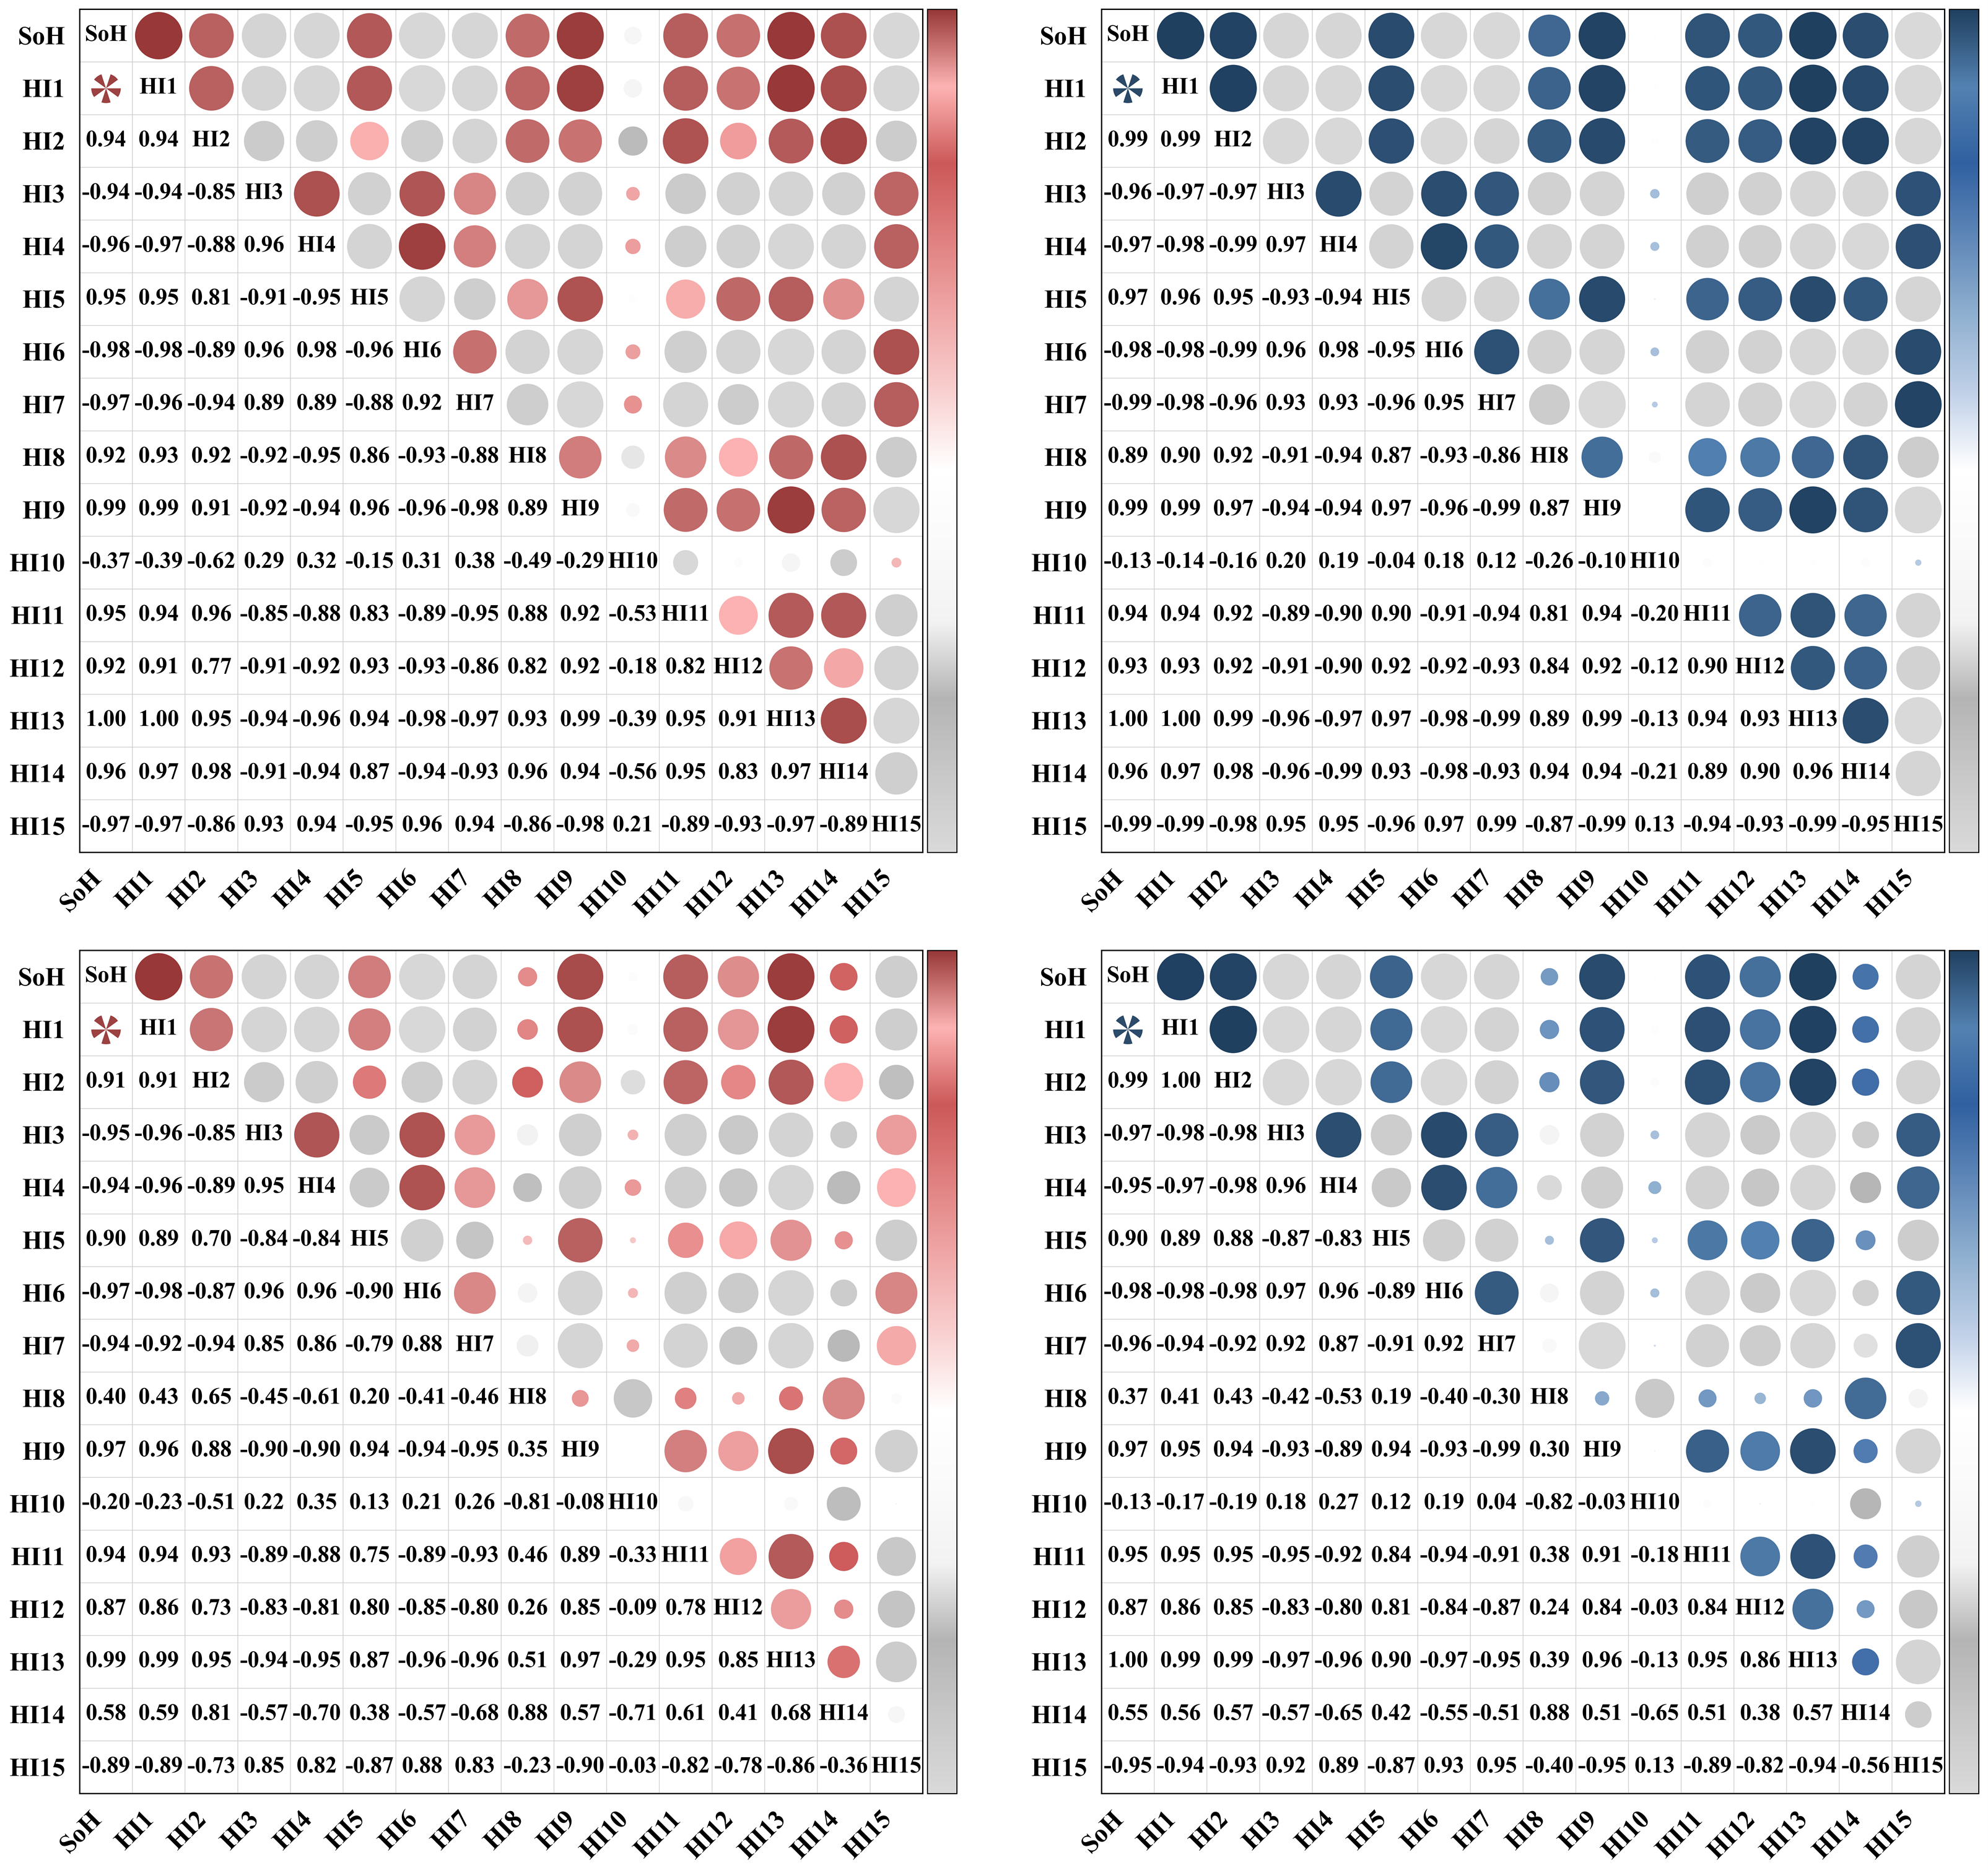
\includegraphics[width=185mm]{figures/fig4_pccscc_print.png}%
}
\caption{Correlation matrices of candidate HIs and SOH on the Oxford dataset.}
\label{fig:2-4}
\end{figure}


\begin{algorithm}[!htbp]
\caption{PCC/SCC dual-threshold health-indicator selection with redundancy constraints}
\label{alg:2-1}
\raggedright
\zihao{5}
\setlength{\tabcolsep}{3.6pt}
\renewcommand{\arraystretch}{1.08}
\begin{adjustbox}{max width=\linewidth}
\begin{tabularx}{\linewidth}{p{0.11\linewidth}X}
\toprule
行号 & 内容 \\
\midrule
输入 & 候选健康指标集合 $\mathcal{F}$；特征开发电池集合 $\mathcal{B}$；各候选指标在特征开发电池上的特征序列及对应SOH序列；阈值 $\theta_{\mathrm{mono}}=0.96$、$\theta_{\mathrm{lin}}=0.92$、$\theta_{\mathrm{co}}=0.95$ \\
输出 & 最终入选健康指标集合 $\mathcal{S}$ \\
1 & 初始化候选集合 $\mathcal{C}=\varnothing$，最终入选集合 $\mathcal{S}=\varnothing$ \\
2 & For 每个候选指标 $f_i\in\mathcal{F}$ do \\
3 & 计算组内最小单调相关性：$mSCC_i=\min_j|\rho_{i,j}|$ \\
4 & 计算组内最小线性相关性：$mPCC_i=\min_j|\gamma_{i,j}|$ \\
5 & If $mSCC_i\geq\theta_{\mathrm{mono}}$ 且 $mPCC_i\geq\theta_{\mathrm{lin}}$ then \\
6 & 将 $f_i$ 加入候选集合 $\mathcal{C}$ \\
7 & End If \\
8 & End For \\
9 & 按 $R_i=\max(mPCC_i,mSCC_i)$ 对 $\mathcal{C}$ 降序排序 \\
10 & For 排序后的每个候选指标 $f_i\in\mathcal{C}$ do \\
11 & 计算 $f_i$ 与每个已入选指标 $f_s\in\mathcal{S}$ 的组平均交叉相关绝对值 $\Phi_{\mathrm{PCC}}(i,s)$ 和 $\Phi_{\mathrm{SCC}}(i,s)$ \\
12 & If 存在 $f_s\in\mathcal{S}$ 使 $\Phi_{\mathrm{PCC}}(i,s)\geq\theta_{\mathrm{co}}$ 且 $\Phi_{\mathrm{SCC}}(i,s)\geq\theta_{\mathrm{co}}$ then \\
13 & 判定 $f_i$ 为冗余指标并跳过 \\
14 & Else \\
15 & 将 $f_i$ 加入最终入选集合 $\mathcal{S}$ \\
16 & End If \\
17 & End For \\
18 & Return $\mathcal{S}$ \\
\bottomrule
\end{tabularx}
\end{adjustbox}
\end{algorithm}


\begin{table}[!htbp]
\caption{Selected HIs and their correlations.}
\label{tab:2-4}
\centering
\zihao{-5}
\setlength{\tabcolsep}{2.4pt}
\renewcommand{\arraystretch}{1.03}
\begin{ThreePartTable}
\begin{adjustbox}{max width=0.99\linewidth}
\begin{tabularx}{0.99\linewidth}{>{\raggedright\arraybackslash}p{0.17\linewidth}>{\centering\arraybackslash}p{0.11\linewidth}>{\raggedright\arraybackslash}p{0.23\linewidth}>{\centering\arraybackslash}p{0.14\linewidth}>{\centering\arraybackslash}p{0.14\linewidth}}
\toprule
Dataset & Selected HI & Feature-development cell & $\lvert\gamma\rvert$ & $\lvert\rho\rvert$ \\
\midrule
Oxford & HI1 & Cell1 & 0.998759 & 0.998710 \\
       &     & Cell2 & 0.997322 & 0.994447 \\
\addlinespace[0.5pt]
CS2    & HI1 & CS2\_36 & 0.990838 & 0.986319 \\
       &     & CS2\_37 & 0.990286 & 0.980124 \\
       & HI2 & CS2\_36 & 0.940029 & 0.989905 \\
       &     & CS2\_37 & 0.938326 & 0.988319 \\
\addlinespace[0.5pt]
CX2    & HI13 & CX2\_36 & 0.999080 & 0.998532 \\
       &      & CX2\_37 & 0.997987 & 0.996442 \\
\addlinespace[0.5pt]
MIT/Severson & HI14 & b3c8  & 0.972972 & 0.995614 \\
             &      & b3c13 & 0.970917 & 0.997651 \\
             & HI15 & b3c8  & 0.979188 & 0.988926 \\
             &      & b3c13 & 0.994096 & 0.995717 \\
\bottomrule
\end{tabularx}
\end{adjustbox}
\end{ThreePartTable}
\end{table}


\begin{table}[!htbp]
\caption{Correlations of selected HIs on independent cells.}
\label{tab:2-5}
\centering
\zihao{-5}
\setlength{\tabcolsep}{2.8pt}
\renewcommand{\arraystretch}{1.05}
\begin{ThreePartTable}
\begin{adjustbox}{max width=0.98\linewidth}
\begin{tabularx}{0.98\linewidth}{>{\raggedright\arraybackslash}p{0.17\linewidth}>{\centering\arraybackslash}p{0.12\linewidth}>{\centering\arraybackslash}p{0.17\linewidth}>{\centering\arraybackslash}p{0.17\linewidth}}
\toprule
Cell & Selected HI & $\lvert\gamma\rvert$ & $\lvert\rho\rvert$ \\
\midrule
Cell3 & HI1 & 0.999052 & 0.999672 \\
Cell4 & HI1 & 0.998933 & 0.999884 \\
Cell5 & HI1 & 0.997874 & 1.000000 \\
Cell6 & HI1 & 0.998257 & 0.999877 \\
Cell7 & HI1 & 0.999337 & 0.999606 \\
Cell8 & HI1 & 0.999259 & 0.999699 \\
CS2\_38 & HI1 & 0.986076 & 0.974359 \\
CS2\_38 & HI2 & 0.932937 & 0.986793 \\
CX2\_38 & HI13 & 0.999576 & 0.999062 \\
b3c29 & HI14 & 0.973516 & 0.996569 \\
b3c29 & HI15 & 0.990303 & 0.992179 \\
\bottomrule
\end{tabularx}
\end{adjustbox}
\end{ThreePartTable}
\end{table}


\begin{table}
\TableStyle
\caption[Absolute PCC comparison of different HIs on the Oxford dataset]{Absolute PCC comparison of different HIs on the Oxford dataset.}
\label{tab:2-6}
\begin{tabularx}{\linewidth}{@{\extracolsep{\fill}}L{0.65}C{0.95}C{1.20}C{0.80}C{0.80}C{1.40}C{1.20}@{}}
\toprule
Cell & HI & \makecell[c]{Sample entropy\\\cite{ref67}} & \makecell[c]{$PP_{\mathrm{DTV}}$\\\cite{ref68}} & \makecell[c]{$P_{\mathrm{IC}}$\\\cite{ref68}} & \makecell[c]{DTV peak position\\$FV_6$\cite{ref69}} & \makecell[c]{Voltage slope\\\cite{ref70}} \\
\midrule
Cell3 & \textbf{0.999052} & 0.9876 & 0.9393 & 0.9729 & 0.964 & 0.9980 \\
Cell4 & \textbf{0.998933} & 0.9885 & 0.9102 & 0.9817 & 0.972 & — \\
Cell5 & \textbf{0.997874} & 0.9133 & 0.9574 & 0.9034 & — & — \\
Cell6 & \textbf{0.998257} & 0.9848 & 0.9299 & 0.9788 & — & — \\
Cell7 & \textbf{0.999337} & 0.9896 & 0.9676 & 0.9748 & 0.983 & 0.9982 \\
Cell8 & \textbf{0.999259} & 0.9908 & 0.9654 & 0.9713 & 0.981 & 0.9979 \\
\bottomrule
\end{tabularx}
\TableNote{Note: Voltage slope denotes the slope of the charging-voltage curve. An em dash indicates that the corresponding correlation coefficient was not reported in the cited study.}
\end{table}


注：“—”表示原文未报告相应电池的相关系数。
